%!TEX root = ../swiatlow_thesis.tex
\label{chapter:jet-reconstruction}


Jet reconstruction in ATLAS makes use of the algorithms described in~\ref{chapter:jets-and-substructure} to create 4-vectors and other observables usable for physics analysis. As previously discussed, a wide variety of algorithms, with various uses and benefits compared to others, are available in the literature. ATLAS most typically makes use of:

\begin{enumerate}
	\item \antikt with $R = 0.4$
	\item \antikt with $R = 0.6$
	\item \antikt with $R = 1.0$, using Trimming with $\Rsub = 0.3$, $\fcut = 5\%$
\end{enumerate}
%
Some analyses also make use of various \CAFat jets, with various forms of split-filtering or reclustered-mass-drop filtering \editnote{Cite these.}. The analyses presented in in this thesis utilize the first and third algorithms, and most of the discussion that follows will focus on various aspects of the reconstruction of these jets.

There are many more aspects to creating a jet than just choosing an algorithm, and this chapter covers the various aspects of jet reconstruction from inputs to calibrations and flavor identification. 

\section{Jet Inputs}


One of the most important decisions in constructing a jet is the decision of what to actually input to the jet algorithm-- i.e., the choice of what to cluster. Several inputs are available, summarized in Figure~\ref{fig:jet-reconstruction:making-jets}. 

%%%%%%%%%%%%%%%%

\begin{figure}
\centering
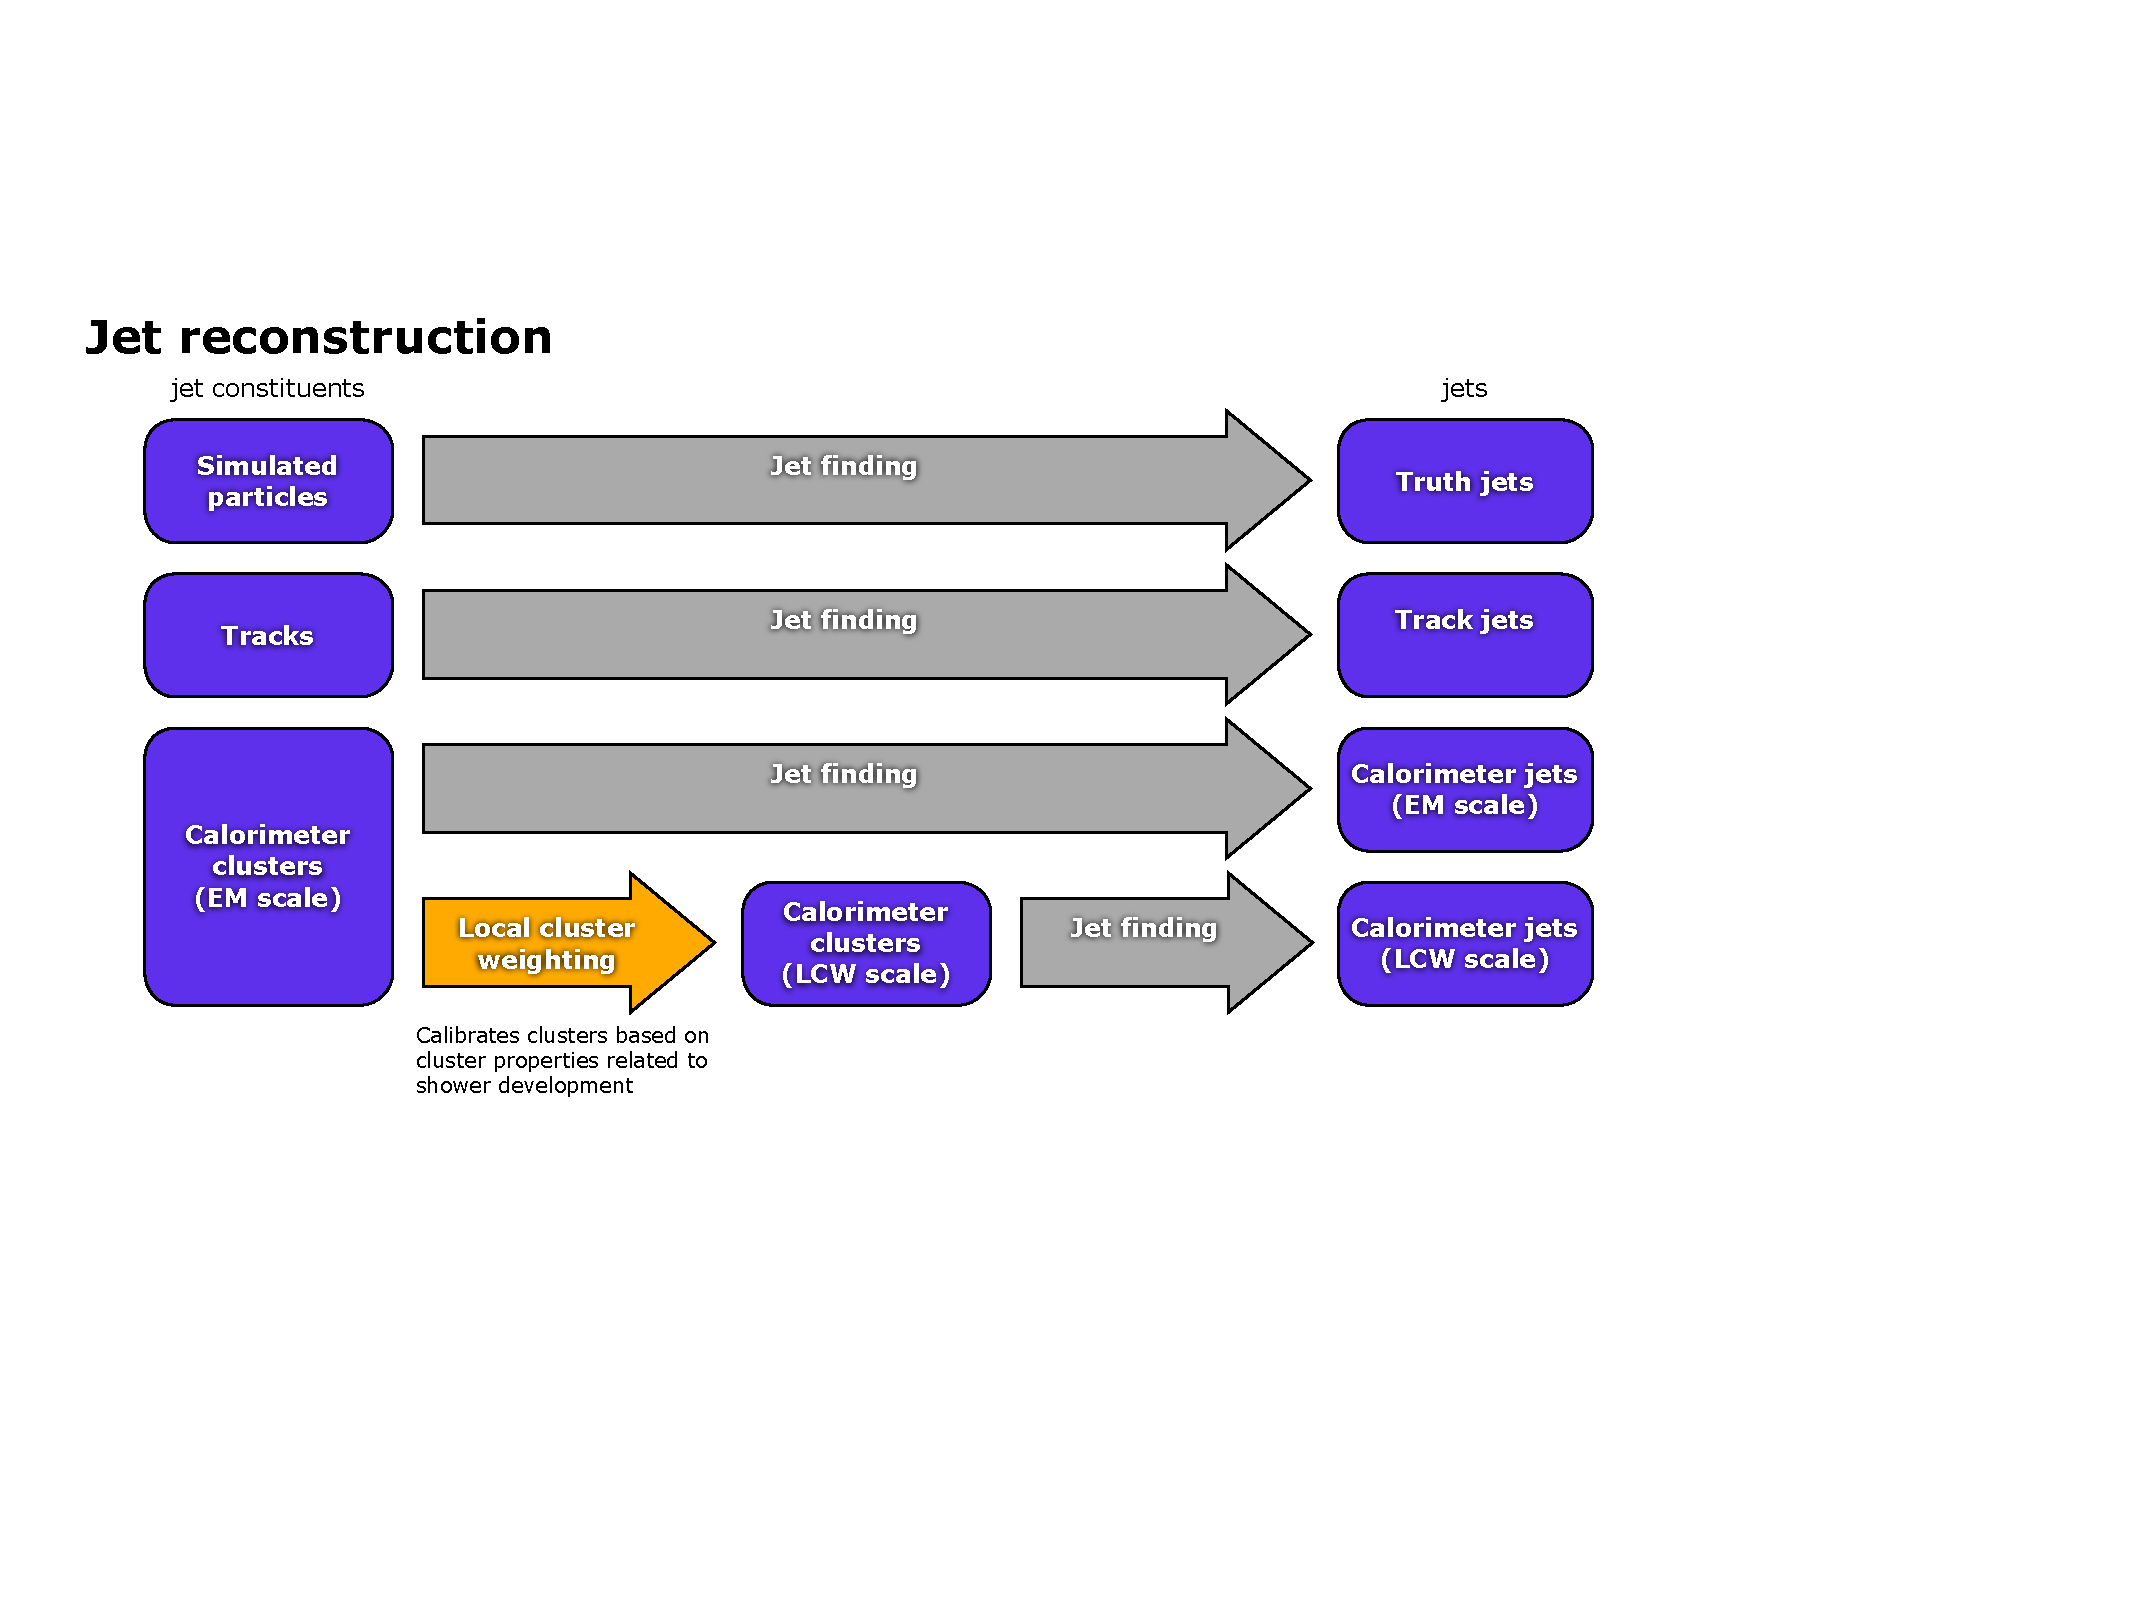
\includegraphics[width=0.7\textwidth]{making-jets.pdf}
\label{fig:jet-reconstruction:making-jets}
\caption{A diagram showing the various forms of jet inputs, and the different types of jets they are used to make.}
\end{figure}

%%%%%%%%%%%%%%%% 

Jets constructed from the simulated particles from a Monte Carlo generator are called \textit{truth jets}: these are primarily used to study the performance of algorithms without the effect of the detector, and to calibrate and define the resolution of other classes of jets. 

Jets can also be constructed from tracks, the outputs of pattern recognition algorithms performed on the hits in the Inner Detector, which correspond to the trajectories of charged particles. These \textit{track jets} are mostly used for validation: they provide a completely independent measurement of a jet from the calorimeter, and while they miss the neutral third of particles, the increased angular precision of tracking can result in complementary information to the calorimeter measurement. \editnote{Cite Seth's thesis, substructure paper?} 

Finally, and most importantly, jets can be formed from energy deposits left in the calorimeter, and these are called \textit{calorimeter jets}. Historically, ATLAS went through many different options for reducing the calorimeter information to a more manageable form for input to jet algorithms-- algorithms such as Global Cell Weighting, Noise Suppressed Towers, and simple projective towers were all eventually disfavored compared to the topo-clustering algorithm described in Section~\ref{jet-reconstruction:jet-inputs:topoclustering}. Calorimeter measurements all share several properties: they provide a measurement of the total energy of the parton shower, produced in both neutral and charged particles. This measurement of the jet (after relevant calibrations are applied) is at approximately the same scale as the quark which initiated it: for example, the invariant mass of the leading non-$b$-tagged jets in semi-leptonic $t\bar{t}$ peaks at the value of the mass of the $W$-boson, $m_{W} = 80$~GeV. Calorimeter jets can thus be used as 4-vectors in the same way that other detector objects-- electrons, photons, etc.-- are used (though of course there is more information in the structure of these jets, which analyses in this thesis do exploit).  \editnote{so many citations needed}

One alternative to separate tracking and calorimeter reconstructions of jets is to use a ``particle flow'' algorithm to combine the measurements from the separate detectors into coherent particle candidates which an be used as inputs to jet algorithms. Such algorithms exploit the fact that charged particles are much more accurately measured (up to some crossing point determined by the strength of the magnetic field) by tracking systems rather than calorimeter systems. Typically, tracks are extrapolated to the calorimeter and matched to energy deposits there; these matched deposits are then subtracted from the calorimeter, as the energy is already accounted for by the tracker. Unmatched energy deposits are assumed to have been created by photons or neutral hadrons, and remain in the list of inputs. Thus, the best features of tracker measurements (accurate energy resolution, and very good angular precision) and calorimeter measurements (capability of measuring neutral particles, good energy resolution at high energies) are combined. The CMS detector is particularly well suited to such reconstruction: the calorimeters are inside the 3.8 T magnetic field (nearly two times stronger than ATLAS), so energy deposits are more widely separated and track-to-calorimeter matching is less ambiguous. Since two thirds of the particles in the jet are reconstructed with tracks instead of calorimeter measurements, the reduced performance of the CMS hadronic calorimeters is also less important. However, as ATLAS has a weaker (and smaller, spatially) magnetic field, and compartively stronger hadronic calorimeters, the improvement from this approached is much diminished and ATLAS has thus far not used the particle flow algorithm for analyses. \editnote{cite cite cite}

The following subsections describe some details of the topoclustering and tracking algorithms which form the inputs to the jet algorithms in ATLAS. The design decisions in these algorithms-- and the strong performance they achieve in the face of difficult operating conditions-- are critical for the final results of hadronic analyses on ATLAS.

\subsection{Topoclustering}
\label{jet-reconstruction:jet-inputs:topoclustering}

\subsection{Tracking}

Discussion of bending, out of cone

\subsubsection{Ghost Association}

Alternative to independent track jets

\subsection{Cluster Calibration}

\section{Jet Calibration}

Once a jet has been clustered, from either EM-scale or LC-scale constituents, it is not yet ready for use by analyses. The non-compensating nature of the ATLAS calorimeters guarantees that the energy measured by the detectors is not the full energy of the particles which passed through them. Jets on ATLAS therefore go through several stages of additional corrections and calibrations, as outlined in Figure~\ref{fig:jet-reconstruction:making-jets}. Each level of the corrections and calibrations is referred to as a \textit{scale}. The steps involved are:

\begin{enumerate}
	\item Jet clustering, producing jets at the \textit{constituent scale} (or EM/LC)
	\item Jet areas pileup correction
	\item A residual NPV and $\mu$ dependent offset, producing jets at the \textit{pileup corrected scale}
	\item A Monte Carlo based \textit{Jet Energy Scale} (JES) calibration, producing jets at the \textit{particle scale}
	\item A Global Sequential Calibration to reduce flavor dependence
	\item In-situ data-driven calibrations, producing jets at the \textit{fully calibrated scale}
\end{enumerate}

All of these steps are applied in ATLAS to $R=0.4$ and $R=0.6$ jets, using both EM and LC-scale inputs. While the LC calibration of the clusters is able to correct for non-compensation to some extent (by noting the difference between hadronic and electromagnetic interactions in the calorimeter, and the corresponding different energies they deposit), even LC-scale jets require significant further calibrations to correspond to truth jets. \LargeR jets, as used by the analyses in this thesis, undergo only the MC JES calibration, for reasons discussed below. The following sections describe each of these steps in detail.

\subsection{Pileup Corrections}

The first stage of jet calibration is to correct for pileup. As the calorimeter has a poor pointing resolution\footnote{Except with the notable exception of the ECal presampler, though this information is still limited and not yet used for pileup identification.}, it is not possible to determine which primary vertex (the hard-scatter, or pileup) an energy deposit originated from. This means that as a calorimeter jet is clustered, it contains energy from both the interaction of interest and the additional less-interesting interactions which occurred during the same bunch crossing. Even if a particle-flow algorithm is used to replace charged hadrons with their tracker measurements, thereby allowing a charged-hadron subtraction using the vertex identification of the tracks, neutral pileup particles cannot be subtracted and will add energy to the jet. \editnote{cite cite}

Jet pileup corrections are a broad topic of active research in both the theoretical and experimental community. \editnote{cite cite} The approach currently used by ATLAS is referred to as the \textit{jet areas} technique~\cite{jetareas}. The basic approach is to measure, event-by-event, the \textit{energy density} $\rho$ in the calorimeter. Though the underlying event contributes, at moderate and higher ($\mu > 10$, approximately) numbers of interactions, the contribution due to pileup to the energy density is dominant. Once the event energy density is measured, and the \textit{jet area} is measured, it is a simple matter to multiply the two and subtract off the pileup contribution to a jet.

The energy density can be measured in many ways. One approach, currently favored in the theory community, is simply to use sliding grid-shaped windows to scan the calorimeter, measuring the total energy deposit in each window, and then taking the median. The median is the best estimate of the ambient energy: measures such as the mean can be biased by the actual hard-scatter jets in the event. The approach used by ATLAS is similar, and follows an older prescription from the authors: the event is clustered into \kt $R=0.4$ jets, and each of their areas is calculated using the \textit{voronoi} technique (described below). The energy/area is calculated for each jet, and the median is used as the energy density (again in order to exclude outliers from real jets).

One detail of the topo-clustering algorithm creates an interesting effect when calculating the energy density. At approximately $\eta = 2.5$, the detector transitions from the barrel to the end-caps, which have a much higher expected noise due to pileup, as discussed in Section~\ref{jet-reconstruction:jet-inputs:topoclustering}. This, along with the reduced granularity in the forward regions, means that the energy density outside of jets decreases substantially: jets themselves are often still energetic enough to go over the noise thresholds required for topocluster formation, but pileup is often not. Thus, when calculating $\rho$, it is important to exclude the forward region of the detector, as the ambient energy outside of jets has greatly different characteristics than in the central region.

There are also several ways of calculating the area of jets, the simplest of which is the voronoi technique previously mentioned. A voronoi algorithm tiles a space (the calorimeter in $y/\phi$ space, in this case) such that each tile contains only one element (i.e., only one topocluster), and each tile contains all the points that are closest to that tile's element compared to any other~\cite{catchmentarea}. The voronoi area has the advantage of being fast to calculate, and gives (on average) the same value as more expensive calculations. The largest issue is that the algorithm does not take into account the energy of each element, which does not reflect the fact that the $k_T$ distance metrics generally do use energy.

A more sophisticated 

Area definitions


\subsection{MC Jet Energy Scale}

\subsection{Global Sequential Calibration}

\subsection{In-situ Calibrations}

\subsection{\LargeR Calibrations}


%%%%%%%%%%%%%%%%

\begin{figure}
\centering
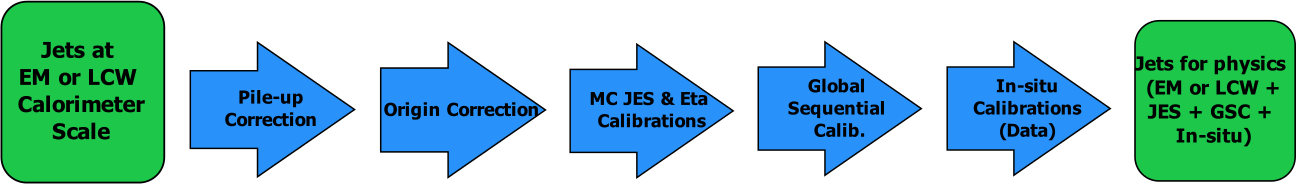
\includegraphics[width=\textwidth]{JES_calib_chain.png}
\label{fig:jet-reconstruction:making-jets}
\caption{A diagram displaying the multiple steps which are used to transform a jet at the constituent scale to a fully-calibrated physics object for use in analysis.}
\end{figure}

%%%%%%%%%%%%%%%% 

\section{Pileup Jet Tagging}
\label{jet-reconstruction:pileup-jet-tagging}

\section{Flavor Tagging}

\section{Quark/Gluon Discrimination}
	\subsection{Lots of subsections}
		...